\documentclass[twoside]{book}

% Packages required by doxygen
\usepackage{fixltx2e}
\usepackage{calc}
\usepackage{doxygen}
\usepackage[export]{adjustbox} % also loads graphicx
\usepackage{graphicx}
\usepackage[utf8]{inputenc}
\usepackage{makeidx}
\usepackage{multicol}
\usepackage{multirow}
\PassOptionsToPackage{warn}{textcomp}
\usepackage{textcomp}
\usepackage[nointegrals]{wasysym}
\usepackage[table]{xcolor}

% Font selection
\usepackage[T1]{fontenc}
\usepackage[scaled=.90]{helvet}
\usepackage{courier}
\usepackage{amssymb}
\usepackage{sectsty}
\renewcommand{\familydefault}{\sfdefault}
\allsectionsfont{%
  \fontseries{bc}\selectfont%
  \color{darkgray}%
}
\renewcommand{\DoxyLabelFont}{%
  \fontseries{bc}\selectfont%
  \color{darkgray}%
}
\newcommand{\+}{\discretionary{\mbox{\scriptsize$\hookleftarrow$}}{}{}}

% Page & text layout
\usepackage{geometry}
\geometry{%
  a4paper,%
  top=2.5cm,%
  bottom=2.5cm,%
  left=2.5cm,%
  right=2.5cm%
}
\tolerance=750
\hfuzz=15pt
\hbadness=750
\setlength{\emergencystretch}{15pt}
\setlength{\parindent}{0cm}
\setlength{\parskip}{3ex plus 2ex minus 2ex}
\makeatletter
\renewcommand{\paragraph}{%
  \@startsection{paragraph}{4}{0ex}{-1.0ex}{1.0ex}{%
    \normalfont\normalsize\bfseries\SS@parafont%
  }%
}
\renewcommand{\subparagraph}{%
  \@startsection{subparagraph}{5}{0ex}{-1.0ex}{1.0ex}{%
    \normalfont\normalsize\bfseries\SS@subparafont%
  }%
}
\makeatother

% Headers & footers
\usepackage{fancyhdr}
\pagestyle{fancyplain}
\fancyhead[LE]{\fancyplain{}{\bfseries\thepage}}
\fancyhead[CE]{\fancyplain{}{}}
\fancyhead[RE]{\fancyplain{}{\bfseries\leftmark}}
\fancyhead[LO]{\fancyplain{}{\bfseries\rightmark}}
\fancyhead[CO]{\fancyplain{}{}}
\fancyhead[RO]{\fancyplain{}{\bfseries\thepage}}
\fancyfoot[LE]{\fancyplain{}{}}
\fancyfoot[CE]{\fancyplain{}{}}
\fancyfoot[RE]{\fancyplain{}{\bfseries\scriptsize Generated by Doxygen }}
\fancyfoot[LO]{\fancyplain{}{\bfseries\scriptsize Generated by Doxygen }}
\fancyfoot[CO]{\fancyplain{}{}}
\fancyfoot[RO]{\fancyplain{}{}}
\renewcommand{\footrulewidth}{0.4pt}
\renewcommand{\chaptermark}[1]{%
  \markboth{#1}{}%
}
\renewcommand{\sectionmark}[1]{%
  \markright{\thesection\ #1}%
}

% Indices & bibliography
\usepackage{natbib}
\usepackage[titles]{tocloft}
\setcounter{tocdepth}{3}
\setcounter{secnumdepth}{5}
\makeindex

% Hyperlinks (required, but should be loaded last)
\usepackage{ifpdf}
\ifpdf
  \usepackage[pdftex,pagebackref=true]{hyperref}
\else
  \usepackage[ps2pdf,pagebackref=true]{hyperref}
\fi
\hypersetup{%
  colorlinks=true,%
  linkcolor=blue,%
  citecolor=blue,%
  unicode%
}

% Custom commands
\newcommand{\clearemptydoublepage}{%
  \newpage{\pagestyle{empty}\cleardoublepage}%
}

\usepackage{caption}
\captionsetup{labelsep=space,justification=centering,font={bf},singlelinecheck=off,skip=4pt,position=top}

%===== C O N T E N T S =====

\begin{document}

% Titlepage & ToC
\hypersetup{pageanchor=false,
             bookmarksnumbered=true,
             pdfencoding=unicode
            }
\pagenumbering{roman}
\begin{titlepage}
\vspace*{7cm}
\begin{center}%
{\Large Traffic Light Client }\\
\vspace*{1cm}
{\large Generated by Doxygen 1.8.11}\\
\end{center}
\end{titlepage}
\clearemptydoublepage
\tableofcontents
\clearemptydoublepage
\pagenumbering{arabic}
\hypersetup{pageanchor=true}

%--- Begin generated contents ---
\chapter{Hierarchical Index}
\section{Class Hierarchy}
This inheritance list is sorted roughly, but not completely, alphabetically\+:\begin{DoxyCompactList}
\item \contentsline{section}{backend.\+Crypto}{\pageref{classbackend_1_1_crypto}}{}
\item \contentsline{section}{application.\+G\+U\+I\+Controller}{\pageref{classapplication_1_1_g_u_i_controller}}{}
\item \contentsline{section}{application.\+Kickstarter}{\pageref{classapplication_1_1_kickstarter}}{}
\item \contentsline{section}{backend.\+Light}{\pageref{classbackend_1_1_light}}{}
\item \contentsline{section}{backend.\+Traffic\+Light}{\pageref{classbackend_1_1_traffic_light}}{}
\item Application\begin{DoxyCompactList}
\item \contentsline{section}{application.\+T\+L\+Client}{\pageref{classapplication_1_1_t_l_client}}{}
\end{DoxyCompactList}
\end{DoxyCompactList}

\chapter{Class Index}
\section{Class List}
Here are the classes, structs, unions and interfaces with brief descriptions\+:\begin{DoxyCompactList}
\item\contentsline{section}{\hyperlink{classbackend_1_1_crypto}{backend.\+Crypto} }{\pageref{classbackend_1_1_crypto}}{}
\item\contentsline{section}{\hyperlink{classapplication_1_1_g_u_i_controller}{application.\+G\+U\+I\+Controller} }{\pageref{classapplication_1_1_g_u_i_controller}}{}
\item\contentsline{section}{\hyperlink{classapplication_1_1_kickstarter}{application.\+Kickstarter} }{\pageref{classapplication_1_1_kickstarter}}{}
\item\contentsline{section}{\hyperlink{classbackend_1_1_light}{backend.\+Light} }{\pageref{classbackend_1_1_light}}{}
\item\contentsline{section}{\hyperlink{classapplication_1_1_t_l_client}{application.\+T\+L\+Client} }{\pageref{classapplication_1_1_t_l_client}}{}
\item\contentsline{section}{\hyperlink{classbackend_1_1_traffic_light}{backend.\+Traffic\+Light} }{\pageref{classbackend_1_1_traffic_light}}{}
\end{DoxyCompactList}

\chapter{Class Documentation}
\hypertarget{classbackend_1_1_crypto}{}\section{backend.\+Crypto Class Reference}
\label{classbackend_1_1_crypto}\index{backend.\+Crypto@{backend.\+Crypto}}
\subsection*{Static Public Member Functions}
\begin{DoxyCompactItemize}
\item 
static String \hyperlink{classbackend_1_1_crypto_ac2ec29ce2e2f0539eb5fc8c1269a3870}{encrypt} (String message, String init\+Vector)
\item 
static String \hyperlink{classbackend_1_1_crypto_a78708641a8d9c9c0f107a108d8d9f268}{decrypt} (String encrypted, String init\+Vector)
\item 
static String \hyperlink{classbackend_1_1_crypto_a19e93de444dc2b59291dec9cac957e90}{get\+Random\+IV} ()
\end{DoxyCompactItemize}


\subsection{Detailed Description}
Cryptographic class.

This class is used to decrypt and encrypt the input and output from the server/client using an A\+ES with an 128-\/bit key. It has a symmetrical key as seen below and will use a random generated 16-\/byte IV which is sent with the message to always output different encrypted results every time.

This will ensure that no one will be able to see the different commands sent by the server/client to interact which means no one can act like the server and send the stop command to the clients without being the server with the correctly encrypted commands. 

\subsection{Member Function Documentation}
\index{backend\+::\+Crypto@{backend\+::\+Crypto}!decrypt@{decrypt}}
\index{decrypt@{decrypt}!backend\+::\+Crypto@{backend\+::\+Crypto}}
\subsubsection[{\texorpdfstring{decrypt(\+String encrypted, String init\+Vector)}{decrypt(String encrypted, String initVector)}}]{\setlength{\rightskip}{0pt plus 5cm}static String backend.\+Crypto.\+decrypt (
\begin{DoxyParamCaption}
\item[{String}]{encrypted, }
\item[{String}]{init\+Vector}
\end{DoxyParamCaption}
)\hspace{0.3cm}{\ttfamily [static]}}\hypertarget{classbackend_1_1_crypto_a78708641a8d9c9c0f107a108d8d9f268}{}\label{classbackend_1_1_crypto_a78708641a8d9c9c0f107a108d8d9f268}
Decrypts the input by using the encrypted text and the IV.

Will first decode the IV into a 16-\/byte array and then use the static symmetric key to decrypt the message through A\+ES. \index{backend\+::\+Crypto@{backend\+::\+Crypto}!encrypt@{encrypt}}
\index{encrypt@{encrypt}!backend\+::\+Crypto@{backend\+::\+Crypto}}
\subsubsection[{\texorpdfstring{encrypt(\+String message, String init\+Vector)}{encrypt(String message, String initVector)}}]{\setlength{\rightskip}{0pt plus 5cm}static String backend.\+Crypto.\+encrypt (
\begin{DoxyParamCaption}
\item[{String}]{message, }
\item[{String}]{init\+Vector}
\end{DoxyParamCaption}
)\hspace{0.3cm}{\ttfamily [static]}}\hypertarget{classbackend_1_1_crypto_ac2ec29ce2e2f0539eb5fc8c1269a3870}{}\label{classbackend_1_1_crypto_ac2ec29ce2e2f0539eb5fc8c1269a3870}
Encrypts input by using the incoming IV and the command.

It uses A\+ES with the static key before returning a Base64 encoded String which makes it easy to decode into bytes again once it is received on the other end. \index{backend\+::\+Crypto@{backend\+::\+Crypto}!get\+Random\+IV@{get\+Random\+IV}}
\index{get\+Random\+IV@{get\+Random\+IV}!backend\+::\+Crypto@{backend\+::\+Crypto}}
\subsubsection[{\texorpdfstring{get\+Random\+I\+V()}{getRandomIV()}}]{\setlength{\rightskip}{0pt plus 5cm}static String backend.\+Crypto.\+get\+Random\+IV (
\begin{DoxyParamCaption}
{}
\end{DoxyParamCaption}
)\hspace{0.3cm}{\ttfamily [static]}}\hypertarget{classbackend_1_1_crypto_a19e93de444dc2b59291dec9cac957e90}{}\label{classbackend_1_1_crypto_a19e93de444dc2b59291dec9cac957e90}
Creates a random IV.

This is used to ensure that the encrypted message is different every single time it is sent. If this wasn\textquotesingle{}t the case it would be easy to see that the same messages are being sent as the encrypted text would be the same every time. 

The documentation for this class was generated from the following file\+:\begin{DoxyCompactItemize}
\item 
T\+L\+Client/src/backend/Crypto.\+java\end{DoxyCompactItemize}

\hypertarget{classapplication_1_1_g_u_i_controller}{}\section{application.\+G\+U\+I\+Controller Class Reference}
\label{classapplication_1_1_g_u_i_controller}\index{application.\+G\+U\+I\+Controller@{application.\+G\+U\+I\+Controller}}
\subsection*{Public Member Functions}
\begin{DoxyCompactItemize}
\item 
void \hyperlink{classapplication_1_1_g_u_i_controller_ab633aa7b0d15917ec268a9a98affe53e}{connect} (Action\+Event event)
\item 
void \hyperlink{classapplication_1_1_g_u_i_controller_a560f50480318cf3c026e748e9d0e175d}{disconnect} (Action\+Event event)
\item 
void {\bfseries disconnect} ()\hypertarget{classapplication_1_1_g_u_i_controller_a1f23ccf4e55ce4a5a6ddcd86d090d3db}{}\label{classapplication_1_1_g_u_i_controller_a1f23ccf4e55ce4a5a6ddcd86d090d3db}

\end{DoxyCompactItemize}
\subsection*{Static Public Member Functions}
\begin{DoxyCompactItemize}
\item 
static void {\bfseries change\+Connection\+Buttons} (boolean \hyperlink{classapplication_1_1_g_u_i_controller_ab633aa7b0d15917ec268a9a98affe53e}{connect})\hypertarget{classapplication_1_1_g_u_i_controller_aa1c5b4085059ed56807425692e87e608}{}\label{classapplication_1_1_g_u_i_controller_aa1c5b4085059ed56807425692e87e608}

\end{DoxyCompactItemize}
\subsection*{Public Attributes}
\begin{DoxyCompactItemize}
\item 
Button {\bfseries button\+\_\+connect}\hypertarget{classapplication_1_1_g_u_i_controller_a6ade76f171c517d12818262a6acf22f9}{}\label{classapplication_1_1_g_u_i_controller_a6ade76f171c517d12818262a6acf22f9}

\item 
Button {\bfseries button\+\_\+disconnect}\hypertarget{classapplication_1_1_g_u_i_controller_adf0551f395ff11e60c5587ddd6c052ef}{}\label{classapplication_1_1_g_u_i_controller_adf0551f395ff11e60c5587ddd6c052ef}

\item 
Image\+View {\bfseries image\+\_\+current\+Light}\hypertarget{classapplication_1_1_g_u_i_controller_aecfe62ae1040631b8963cbc2633b4dd5}{}\label{classapplication_1_1_g_u_i_controller_aecfe62ae1040631b8963cbc2633b4dd5}

\end{DoxyCompactItemize}
\subsection*{Static Public Attributes}
\begin{DoxyCompactItemize}
\item 
static Button {\bfseries sbutton\+\_\+connect}\hypertarget{classapplication_1_1_g_u_i_controller_a7e58633df5cb9f7992ea250f126363d0}{}\label{classapplication_1_1_g_u_i_controller_a7e58633df5cb9f7992ea250f126363d0}

\item 
static Radio\+Button {\bfseries sradio\+\_\+standard}\hypertarget{classapplication_1_1_g_u_i_controller_a8daa294d1887172f654fdb68bbe7f98e}{}\label{classapplication_1_1_g_u_i_controller_a8daa294d1887172f654fdb68bbe7f98e}

\end{DoxyCompactItemize}


\subsection{Detailed Description}
Java\+FX controller to control the Scene Builder created user interface. 

\subsection{Member Function Documentation}
\index{application\+::\+G\+U\+I\+Controller@{application\+::\+G\+U\+I\+Controller}!connect@{connect}}
\index{connect@{connect}!application\+::\+G\+U\+I\+Controller@{application\+::\+G\+U\+I\+Controller}}
\subsubsection[{\texorpdfstring{connect(\+Action\+Event event)}{connect(ActionEvent event)}}]{\setlength{\rightskip}{0pt plus 5cm}void application.\+G\+U\+I\+Controller.\+connect (
\begin{DoxyParamCaption}
\item[{Action\+Event}]{event}
\end{DoxyParamCaption}
)}\hypertarget{classapplication_1_1_g_u_i_controller_ab633aa7b0d15917ec268a9a98affe53e}{}\label{classapplication_1_1_g_u_i_controller_ab633aa7b0d15917ec268a9a98affe53e}
Button event when the button\+\_\+connect is pressed.

Connects the client by creating the bridge between the Traffic Light and the G\+UI and sending user interface related information from the host field, the port field and type fields. While also sending the imageview further down the classes. \index{application\+::\+G\+U\+I\+Controller@{application\+::\+G\+U\+I\+Controller}!disconnect@{disconnect}}
\index{disconnect@{disconnect}!application\+::\+G\+U\+I\+Controller@{application\+::\+G\+U\+I\+Controller}}
\subsubsection[{\texorpdfstring{disconnect(\+Action\+Event event)}{disconnect(ActionEvent event)}}]{\setlength{\rightskip}{0pt plus 5cm}void application.\+G\+U\+I\+Controller.\+disconnect (
\begin{DoxyParamCaption}
\item[{Action\+Event}]{event}
\end{DoxyParamCaption}
)}\hypertarget{classapplication_1_1_g_u_i_controller_a560f50480318cf3c026e748e9d0e175d}{}\label{classapplication_1_1_g_u_i_controller_a560f50480318cf3c026e748e9d0e175d}
Button event when the button\+\_\+disconnect is pressed.

Disconnects the client by stopping the threads and nulling the bridge killing off the client\textquotesingle{}s connection completely. Also reenables the connect button by using the workaround. 

The documentation for this class was generated from the following file\+:\begin{DoxyCompactItemize}
\item 
T\+L\+Client/src/application/G\+U\+I\+Controller.\+java\end{DoxyCompactItemize}

\hypertarget{classapplication_1_1_kickstarter}{}\section{application.\+Kickstarter Class Reference}
\label{classapplication_1_1_kickstarter}\index{application.\+Kickstarter@{application.\+Kickstarter}}
\subsection*{Public Member Functions}
\begin{DoxyCompactItemize}
\item 
\hyperlink{classapplication_1_1_kickstarter_a967b3fbe01bc93fef2821741613d0db7}{Kickstarter} (String hostname, int \+\_\+port, boolean walk, Image\+View view)
\item 
void \hyperlink{classapplication_1_1_kickstarter_a13fc6c3b4b32c29af30649cf387a5bc0}{connect} ()
\item 
void \hyperlink{classapplication_1_1_kickstarter_ab4c9b1c4909606883afeff6552d2bd8b}{disconnect} ()
\end{DoxyCompactItemize}


\subsection{Detailed Description}
This class is meant as a bridge between the G\+UI Controller and the Traffic Light.

The reason for this being the Main class (\hyperlink{classapplication_1_1_t_l_client}{T\+L\+Client}) is mainly used to initialize the G\+UI and its Java\+FX controller, thus in order to separate the G\+UI controller and what actually starts the client backend, this acts like the main method to kickstart the client instead of handling client objects inside the G\+UI controller. 

\subsection{Constructor \& Destructor Documentation}
\index{application\+::\+Kickstarter@{application\+::\+Kickstarter}!Kickstarter@{Kickstarter}}
\index{Kickstarter@{Kickstarter}!application\+::\+Kickstarter@{application\+::\+Kickstarter}}
\subsubsection[{\texorpdfstring{Kickstarter(\+String hostname, int \+\_\+port, boolean walk, Image\+View view)}{Kickstarter(String hostname, int _port, boolean walk, ImageView view)}}]{\setlength{\rightskip}{0pt plus 5cm}application.\+Kickstarter.\+Kickstarter (
\begin{DoxyParamCaption}
\item[{String}]{hostname, }
\item[{int}]{\+\_\+port, }
\item[{boolean}]{walk, }
\item[{Image\+View}]{view}
\end{DoxyParamCaption}
)}\hypertarget{classapplication_1_1_kickstarter_a967b3fbe01bc93fef2821741613d0db7}{}\label{classapplication_1_1_kickstarter_a967b3fbe01bc93fef2821741613d0db7}
Gets the hostname, port and traffic light type as arguments from the G\+UI controller. The Image\+View from the center of the G\+UI is also sent through here in order for the traffic light to get access to this and change it when the lights change. 

\subsection{Member Function Documentation}
\index{application\+::\+Kickstarter@{application\+::\+Kickstarter}!connect@{connect}}
\index{connect@{connect}!application\+::\+Kickstarter@{application\+::\+Kickstarter}}
\subsubsection[{\texorpdfstring{connect()}{connect()}}]{\setlength{\rightskip}{0pt plus 5cm}void application.\+Kickstarter.\+connect (
\begin{DoxyParamCaption}
{}
\end{DoxyParamCaption}
)}\hypertarget{classapplication_1_1_kickstarter_a13fc6c3b4b32c29af30649cf387a5bc0}{}\label{classapplication_1_1_kickstarter_a13fc6c3b4b32c29af30649cf387a5bc0}
Connects to the traffic light using the hostname and the port acquired from the user interface. \index{application\+::\+Kickstarter@{application\+::\+Kickstarter}!disconnect@{disconnect}}
\index{disconnect@{disconnect}!application\+::\+Kickstarter@{application\+::\+Kickstarter}}
\subsubsection[{\texorpdfstring{disconnect()}{disconnect()}}]{\setlength{\rightskip}{0pt plus 5cm}void application.\+Kickstarter.\+disconnect (
\begin{DoxyParamCaption}
{}
\end{DoxyParamCaption}
)}\hypertarget{classapplication_1_1_kickstarter_ab4c9b1c4909606883afeff6552d2bd8b}{}\label{classapplication_1_1_kickstarter_ab4c9b1c4909606883afeff6552d2bd8b}
Disconnects the traffic light by 

The documentation for this class was generated from the following file\+:\begin{DoxyCompactItemize}
\item 
T\+L\+Client/src/application/Kickstarter.\+java\end{DoxyCompactItemize}

\hypertarget{classbackend_1_1_light}{}\section{backend.\+Light Class Reference}
\label{classbackend_1_1_light}\index{backend.\+Light@{backend.\+Light}}
\subsection*{Public Member Functions}
\begin{DoxyCompactItemize}
\item 
\hyperlink{classbackend_1_1_light_ae178ed543c16a272525f125b546bcdc7}{Light} (String \+\_\+name, int freq, String image\+Name)
\item 
Image \hyperlink{classbackend_1_1_light_ad532db1f7e6546f1eb4c760f84d3092f}{get\+Image} ()
\item 
String \hyperlink{classbackend_1_1_light_afb407ae3e7f06bcd31ba9804bf93a650}{get\+Name} ()
\item 
void \hyperlink{classbackend_1_1_light_a3d80e153d8b8040dc407e9a38a7c056a}{frequency} (int new\+Freq)
\item 
int \hyperlink{classbackend_1_1_light_ae6e17df986c1ebb3bb23d551ff56237b}{get\+Frequency} ()
\item 
void \hyperlink{classbackend_1_1_light_a7c32c5e1c8a2e62d3022803ceb31f9cf}{enabled} (boolean bool)
\item 
boolean \hyperlink{classbackend_1_1_light_a012219634e4d5e30adc50b5a96b405b7}{is\+Enabled} ()
\end{DoxyCompactItemize}


\subsection{Detailed Description}
This class contains all the information about the light. This simplifies the Traffic \hyperlink{classbackend_1_1_light}{Light} structure by encapsulating all light information inside a single class that the traffic light manipulates.

There are usually three of these inside the traffic light -\/ red, yellow and green. 

\subsection{Constructor \& Destructor Documentation}
\index{backend\+::\+Light@{backend\+::\+Light}!Light@{Light}}
\index{Light@{Light}!backend\+::\+Light@{backend\+::\+Light}}
\subsubsection[{\texorpdfstring{Light(\+String \+\_\+name, int freq, String image\+Name)}{Light(String _name, int freq, String imageName)}}]{\setlength{\rightskip}{0pt plus 5cm}backend.\+Light.\+Light (
\begin{DoxyParamCaption}
\item[{String}]{\+\_\+name, }
\item[{int}]{freq, }
\item[{String}]{image\+Name}
\end{DoxyParamCaption}
)}\hypertarget{classbackend_1_1_light_ae178ed543c16a272525f125b546bcdc7}{}\label{classbackend_1_1_light_ae178ed543c16a272525f125b546bcdc7}
The default constructor used in the traffic light class.

Has the light\textquotesingle{}s name, frequency and the image representation as parameters. 

\subsection{Member Function Documentation}
\index{backend\+::\+Light@{backend\+::\+Light}!enabled@{enabled}}
\index{enabled@{enabled}!backend\+::\+Light@{backend\+::\+Light}}
\subsubsection[{\texorpdfstring{enabled(boolean bool)}{enabled(boolean bool)}}]{\setlength{\rightskip}{0pt plus 5cm}void backend.\+Light.\+enabled (
\begin{DoxyParamCaption}
\item[{boolean}]{bool}
\end{DoxyParamCaption}
)}\hypertarget{classbackend_1_1_light_a7c32c5e1c8a2e62d3022803ceb31f9cf}{}\label{classbackend_1_1_light_a7c32c5e1c8a2e62d3022803ceb31f9cf}
Sets whether or not the light is lit up. \index{backend\+::\+Light@{backend\+::\+Light}!frequency@{frequency}}
\index{frequency@{frequency}!backend\+::\+Light@{backend\+::\+Light}}
\subsubsection[{\texorpdfstring{frequency(int new\+Freq)}{frequency(int newFreq)}}]{\setlength{\rightskip}{0pt plus 5cm}void backend.\+Light.\+frequency (
\begin{DoxyParamCaption}
\item[{int}]{new\+Freq}
\end{DoxyParamCaption}
)}\hypertarget{classbackend_1_1_light_a3d80e153d8b8040dc407e9a38a7c056a}{}\label{classbackend_1_1_light_a3d80e153d8b8040dc407e9a38a7c056a}
Sets the frequency in seconds for this light. \index{backend\+::\+Light@{backend\+::\+Light}!get\+Frequency@{get\+Frequency}}
\index{get\+Frequency@{get\+Frequency}!backend\+::\+Light@{backend\+::\+Light}}
\subsubsection[{\texorpdfstring{get\+Frequency()}{getFrequency()}}]{\setlength{\rightskip}{0pt plus 5cm}int backend.\+Light.\+get\+Frequency (
\begin{DoxyParamCaption}
{}
\end{DoxyParamCaption}
)}\hypertarget{classbackend_1_1_light_ae6e17df986c1ebb3bb23d551ff56237b}{}\label{classbackend_1_1_light_ae6e17df986c1ebb3bb23d551ff56237b}
Gets the frequency in seconds for this light. \index{backend\+::\+Light@{backend\+::\+Light}!get\+Image@{get\+Image}}
\index{get\+Image@{get\+Image}!backend\+::\+Light@{backend\+::\+Light}}
\subsubsection[{\texorpdfstring{get\+Image()}{getImage()}}]{\setlength{\rightskip}{0pt plus 5cm}Image backend.\+Light.\+get\+Image (
\begin{DoxyParamCaption}
{}
\end{DoxyParamCaption}
)}\hypertarget{classbackend_1_1_light_ad532db1f7e6546f1eb4c760f84d3092f}{}\label{classbackend_1_1_light_ad532db1f7e6546f1eb4c760f84d3092f}
Gets the image for this light. \index{backend\+::\+Light@{backend\+::\+Light}!get\+Name@{get\+Name}}
\index{get\+Name@{get\+Name}!backend\+::\+Light@{backend\+::\+Light}}
\subsubsection[{\texorpdfstring{get\+Name()}{getName()}}]{\setlength{\rightskip}{0pt plus 5cm}String backend.\+Light.\+get\+Name (
\begin{DoxyParamCaption}
{}
\end{DoxyParamCaption}
)}\hypertarget{classbackend_1_1_light_afb407ae3e7f06bcd31ba9804bf93a650}{}\label{classbackend_1_1_light_afb407ae3e7f06bcd31ba9804bf93a650}
Gets the name for this light. \index{backend\+::\+Light@{backend\+::\+Light}!is\+Enabled@{is\+Enabled}}
\index{is\+Enabled@{is\+Enabled}!backend\+::\+Light@{backend\+::\+Light}}
\subsubsection[{\texorpdfstring{is\+Enabled()}{isEnabled()}}]{\setlength{\rightskip}{0pt plus 5cm}boolean backend.\+Light.\+is\+Enabled (
\begin{DoxyParamCaption}
{}
\end{DoxyParamCaption}
)}\hypertarget{classbackend_1_1_light_a012219634e4d5e30adc50b5a96b405b7}{}\label{classbackend_1_1_light_a012219634e4d5e30adc50b5a96b405b7}
Gets whether or not the light is lit up. 

The documentation for this class was generated from the following file\+:\begin{DoxyCompactItemize}
\item 
T\+L\+Client/src/backend/Light.\+java\end{DoxyCompactItemize}

\hypertarget{classapplication_1_1_t_l_client}{}\section{application.\+T\+L\+Client Class Reference}
\label{classapplication_1_1_t_l_client}\index{application.\+T\+L\+Client@{application.\+T\+L\+Client}}
Inheritance diagram for application.\+T\+L\+Client\+:\begin{figure}[H]
\begin{center}
\leavevmode
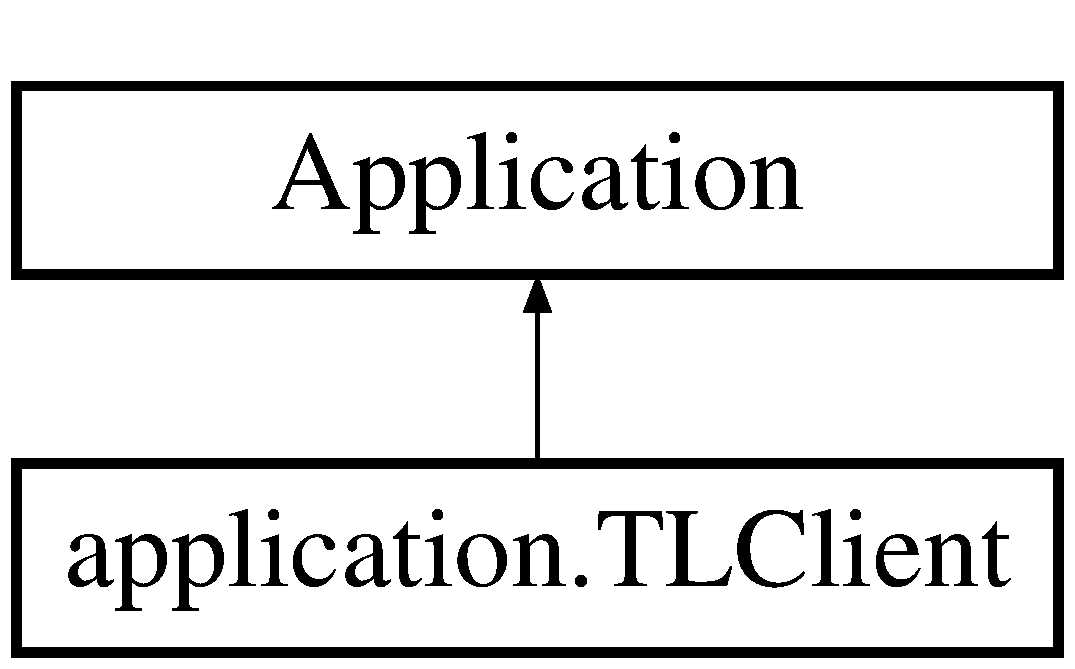
\includegraphics[height=2.000000cm]{classapplication_1_1_t_l_client}
\end{center}
\end{figure}
\subsection*{Public Member Functions}
\begin{DoxyCompactItemize}
\item 
void {\bfseries start} (Stage primary\+Stage)\hypertarget{classapplication_1_1_t_l_client_a079567d06294cf7bc37b2e13c0441574}{}\label{classapplication_1_1_t_l_client_a079567d06294cf7bc37b2e13c0441574}

\item 
void \hyperlink{classapplication_1_1_t_l_client_a13e5e430611f2c89df8b3854843b41ba}{init\+Root\+Layout} ()
\end{DoxyCompactItemize}
\subsection*{Static Public Member Functions}
\begin{DoxyCompactItemize}
\item 
static void {\bfseries main} (String\mbox{[}$\,$\mbox{]} args)\hypertarget{classapplication_1_1_t_l_client_a2b602e35c6c33e4195f031187f90253c}{}\label{classapplication_1_1_t_l_client_a2b602e35c6c33e4195f031187f90253c}

\end{DoxyCompactItemize}


\subsection{Detailed Description}
This is the main class and it basically doesn\textquotesingle{}t do anything except setting up the window using Java\+FX.

Most of the important stuff is done from the \hyperlink{classapplication_1_1_kickstarter}{Kickstarter} class instead of this one. 

\subsection{Member Function Documentation}
\index{application\+::\+T\+L\+Client@{application\+::\+T\+L\+Client}!init\+Root\+Layout@{init\+Root\+Layout}}
\index{init\+Root\+Layout@{init\+Root\+Layout}!application\+::\+T\+L\+Client@{application\+::\+T\+L\+Client}}
\subsubsection[{\texorpdfstring{init\+Root\+Layout()}{initRootLayout()}}]{\setlength{\rightskip}{0pt plus 5cm}void application.\+T\+L\+Client.\+init\+Root\+Layout (
\begin{DoxyParamCaption}
{}
\end{DoxyParamCaption}
)}\hypertarget{classapplication_1_1_t_l_client_a13e5e430611f2c89df8b3854843b41ba}{}\label{classapplication_1_1_t_l_client_a13e5e430611f2c89df8b3854843b41ba}
Sets up the G\+UI using Java\+FX. 

The documentation for this class was generated from the following file\+:\begin{DoxyCompactItemize}
\item 
T\+L\+Client/src/application/T\+L\+Client.\+java\end{DoxyCompactItemize}

\hypertarget{classbackend_1_1_traffic_light}{}\section{backend.\+Traffic\+Light Class Reference}
\label{classbackend_1_1_traffic_light}\index{backend.\+Traffic\+Light@{backend.\+Traffic\+Light}}
\subsection*{Public Member Functions}
\begin{DoxyCompactItemize}
\item 
\hyperlink{classbackend_1_1_traffic_light_a68941f8d3b0bbff67b69f3c189d77788}{Traffic\+Light} (Image\+View \+\_\+view, boolean walk\+\_\+)
\item 
void \hyperlink{classbackend_1_1_traffic_light_a4dfc82eed9125fee41834447918ecafe}{set\+Light\+Frequency} (int colour, int seconds)
\item 
int {\bfseries get\+Light\+Frequency} (int colour)\hypertarget{classbackend_1_1_traffic_light_afb34bdb3be2f60a76111ed774480ae01}{}\label{classbackend_1_1_traffic_light_afb34bdb3be2f60a76111ed774480ae01}

\item 
int \hyperlink{classbackend_1_1_traffic_light_a2d0231e3f47fa1003d43069d2dfbf7ec}{get\+Active\+Colour} ()
\item 
boolean {\bfseries get\+Walk} ()\hypertarget{classbackend_1_1_traffic_light_a51494a57afd2d10a8791d29b79540b27}{}\label{classbackend_1_1_traffic_light_a51494a57afd2d10a8791d29b79540b27}

\item 
Callable {\bfseries switch\+Colour} ()\hypertarget{classbackend_1_1_traffic_light_a704ee3bbe733ce6e0e4fbedc9f0794bd}{}\label{classbackend_1_1_traffic_light_a704ee3bbe733ce6e0e4fbedc9f0794bd}

\item 
void \hyperlink{classbackend_1_1_traffic_light_a3189b2b6440789c714bb004cb792d452}{change\+Image} ()
\item 
void {\bfseries change\+Image} (String image)\hypertarget{classbackend_1_1_traffic_light_a353a1c82eadb571e4b982dcab075d2d4}{}\label{classbackend_1_1_traffic_light_a353a1c82eadb571e4b982dcab075d2d4}

\item 
void \hyperlink{classbackend_1_1_traffic_light_a2dae4e4bfeedec1232e759580fbd2f8c}{schedule\+Next} ()
\item 
void \hyperlink{classbackend_1_1_traffic_light_a4dd4e39baf73d8eff0385fd794944eb8}{connect} (String \+\_\+host\+Name, int \+\_\+port)
\item 
void \hyperlink{classbackend_1_1_traffic_light_aee505c8f323e1e2c3663e9a9fe0a90f1}{disconnect} ()
\item 
void \hyperlink{classbackend_1_1_traffic_light_ad84d11094e93d1ca839c97c27ac55f48}{initialize\+Scheduler} (int colour)
\item 
void \hyperlink{classbackend_1_1_traffic_light_a3853f64679ecfcf4c13db7acbaba9c19}{run} ()
\item 
void \hyperlink{classbackend_1_1_traffic_light_a80ff066019e22052573b8ab47c655040}{send} (String s)
\item 
void \hyperlink{classbackend_1_1_traffic_light_ac9f6beaf190c5cb4b50fee8b5e0f909c}{do\+Command} (String decrypted)  throws I\+O\+Exception
\end{DoxyCompactItemize}
\subsection*{Public Attributes}
\begin{DoxyCompactItemize}
\item 
Image\+View {\bfseries view}\hypertarget{classbackend_1_1_traffic_light_a76ecbec9c0244e880c8c849150dbdb69}{}\label{classbackend_1_1_traffic_light_a76ecbec9c0244e880c8c849150dbdb69}

\item 
boolean {\bfseries quit}\hypertarget{classbackend_1_1_traffic_light_ad789b37270d95c493d611d67757987c3}{}\label{classbackend_1_1_traffic_light_ad789b37270d95c493d611d67757987c3}

\item 
Thread {\bfseries tlight\+Thread}\hypertarget{classbackend_1_1_traffic_light_aa8c9e0459fb06dfa8ab52a39b01ff1a2}{}\label{classbackend_1_1_traffic_light_aa8c9e0459fb06dfa8ab52a39b01ff1a2}

\end{DoxyCompactItemize}


\subsection{Detailed Description}
The traffic light class is meant as the actual traffic light or a walking sign.

It consists of three lights -\/ Red, Yellow and Green and is where the client connects with the host. It is here the scheduling is done for the client, and it is here where the server and client communicates. This is also where the images are changed, the frequencies are set and input/output is interpreted. 

\subsection{Constructor \& Destructor Documentation}
\index{backend\+::\+Traffic\+Light@{backend\+::\+Traffic\+Light}!Traffic\+Light@{Traffic\+Light}}
\index{Traffic\+Light@{Traffic\+Light}!backend\+::\+Traffic\+Light@{backend\+::\+Traffic\+Light}}
\subsubsection[{\texorpdfstring{Traffic\+Light(\+Image\+View \+\_\+view, boolean walk\+\_\+)}{TrafficLight(ImageView _view, boolean walk_)}}]{\setlength{\rightskip}{0pt plus 5cm}backend.\+Traffic\+Light.\+Traffic\+Light (
\begin{DoxyParamCaption}
\item[{Image\+View}]{\+\_\+view, }
\item[{boolean}]{walk\+\_\+}
\end{DoxyParamCaption}
)}\hypertarget{classbackend_1_1_traffic_light_a68941f8d3b0bbff67b69f3c189d77788}{}\label{classbackend_1_1_traffic_light_a68941f8d3b0bbff67b69f3c189d77788}
Sets the light to default values\+:

Red\+: 5 seconds Yellow\+: 2 seconds. Green\+: 5 seconds. 

\subsection{Member Function Documentation}
\index{backend\+::\+Traffic\+Light@{backend\+::\+Traffic\+Light}!change\+Image@{change\+Image}}
\index{change\+Image@{change\+Image}!backend\+::\+Traffic\+Light@{backend\+::\+Traffic\+Light}}
\subsubsection[{\texorpdfstring{change\+Image()}{changeImage()}}]{\setlength{\rightskip}{0pt plus 5cm}void backend.\+Traffic\+Light.\+change\+Image (
\begin{DoxyParamCaption}
{}
\end{DoxyParamCaption}
)}\hypertarget{classbackend_1_1_traffic_light_a3189b2b6440789c714bb004cb792d452}{}\label{classbackend_1_1_traffic_light_a3189b2b6440789c714bb004cb792d452}
Switches the image shown on the client\textquotesingle{}s user interface. \index{backend\+::\+Traffic\+Light@{backend\+::\+Traffic\+Light}!connect@{connect}}
\index{connect@{connect}!backend\+::\+Traffic\+Light@{backend\+::\+Traffic\+Light}}
\subsubsection[{\texorpdfstring{connect(\+String \+\_\+host\+Name, int \+\_\+port)}{connect(String _hostName, int _port)}}]{\setlength{\rightskip}{0pt plus 5cm}void backend.\+Traffic\+Light.\+connect (
\begin{DoxyParamCaption}
\item[{String}]{\+\_\+host\+Name, }
\item[{int}]{\+\_\+port}
\end{DoxyParamCaption}
)}\hypertarget{classbackend_1_1_traffic_light_a4dd4e39baf73d8eff0385fd794944eb8}{}\label{classbackend_1_1_traffic_light_a4dd4e39baf73d8eff0385fd794944eb8}
Connects to the server by using the client\+Socket. Will start the traffic light immediately after connection succeeded. \index{backend\+::\+Traffic\+Light@{backend\+::\+Traffic\+Light}!disconnect@{disconnect}}
\index{disconnect@{disconnect}!backend\+::\+Traffic\+Light@{backend\+::\+Traffic\+Light}}
\subsubsection[{\texorpdfstring{disconnect()}{disconnect()}}]{\setlength{\rightskip}{0pt plus 5cm}void backend.\+Traffic\+Light.\+disconnect (
\begin{DoxyParamCaption}
{}
\end{DoxyParamCaption}
)}\hypertarget{classbackend_1_1_traffic_light_aee505c8f323e1e2c3663e9a9fe0a90f1}{}\label{classbackend_1_1_traffic_light_aee505c8f323e1e2c3663e9a9fe0a90f1}
Shuts down the scheduler and the scheduler queue. \index{backend\+::\+Traffic\+Light@{backend\+::\+Traffic\+Light}!do\+Command@{do\+Command}}
\index{do\+Command@{do\+Command}!backend\+::\+Traffic\+Light@{backend\+::\+Traffic\+Light}}
\subsubsection[{\texorpdfstring{do\+Command(\+String decrypted)}{doCommand(String decrypted)}}]{\setlength{\rightskip}{0pt plus 5cm}void backend.\+Traffic\+Light.\+do\+Command (
\begin{DoxyParamCaption}
\item[{String}]{decrypted}
\end{DoxyParamCaption}
) throws I\+O\+Exception}\hypertarget{classbackend_1_1_traffic_light_ac9f6beaf190c5cb4b50fee8b5e0f909c}{}\label{classbackend_1_1_traffic_light_ac9f6beaf190c5cb4b50fee8b5e0f909c}
Completes commands.

Checks the command from a decrypted input. This is sent from the run method. It has three command possibilities\+:
\begin{DoxyItemize}
\item \char`\"{}kill\char`\"{} (server asks this client to shut down).
\item \char`\"{}\+C$\ast$$\ast$$\ast$\char`\"{} (color synchronization. See comments below.)
\item \char`\"{}sync\char`\"{} (stops client, waits for server response to synchronize with other clients). 
\end{DoxyItemize}\index{backend\+::\+Traffic\+Light@{backend\+::\+Traffic\+Light}!get\+Active\+Colour@{get\+Active\+Colour}}
\index{get\+Active\+Colour@{get\+Active\+Colour}!backend\+::\+Traffic\+Light@{backend\+::\+Traffic\+Light}}
\subsubsection[{\texorpdfstring{get\+Active\+Colour()}{getActiveColour()}}]{\setlength{\rightskip}{0pt plus 5cm}int backend.\+Traffic\+Light.\+get\+Active\+Colour (
\begin{DoxyParamCaption}
{}
\end{DoxyParamCaption}
)}\hypertarget{classbackend_1_1_traffic_light_a2d0231e3f47fa1003d43069d2dfbf7ec}{}\label{classbackend_1_1_traffic_light_a2d0231e3f47fa1003d43069d2dfbf7ec}
Goes through the lights and looks for which one is lit at this point. \index{backend\+::\+Traffic\+Light@{backend\+::\+Traffic\+Light}!initialize\+Scheduler@{initialize\+Scheduler}}
\index{initialize\+Scheduler@{initialize\+Scheduler}!backend\+::\+Traffic\+Light@{backend\+::\+Traffic\+Light}}
\subsubsection[{\texorpdfstring{initialize\+Scheduler(int colour)}{initializeScheduler(int colour)}}]{\setlength{\rightskip}{0pt plus 5cm}void backend.\+Traffic\+Light.\+initialize\+Scheduler (
\begin{DoxyParamCaption}
\item[{int}]{colour}
\end{DoxyParamCaption}
)}\hypertarget{classbackend_1_1_traffic_light_ad84d11094e93d1ca839c97c27ac55f48}{}\label{classbackend_1_1_traffic_light_ad84d11094e93d1ca839c97c27ac55f48}
Initializes the scheduler all over again. Because once it is shut down it is unusable until re-\/initialized. This is done when synchronizing and when connecting. \index{backend\+::\+Traffic\+Light@{backend\+::\+Traffic\+Light}!run@{run}}
\index{run@{run}!backend\+::\+Traffic\+Light@{backend\+::\+Traffic\+Light}}
\subsubsection[{\texorpdfstring{run()}{run()}}]{\setlength{\rightskip}{0pt plus 5cm}void backend.\+Traffic\+Light.\+run (
\begin{DoxyParamCaption}
{}
\end{DoxyParamCaption}
)}\hypertarget{classbackend_1_1_traffic_light_a3853f64679ecfcf4c13db7acbaba9c19}{}\label{classbackend_1_1_traffic_light_a3853f64679ecfcf4c13db7acbaba9c19}
Main stuff where all the magic happens. \index{backend\+::\+Traffic\+Light@{backend\+::\+Traffic\+Light}!schedule\+Next@{schedule\+Next}}
\index{schedule\+Next@{schedule\+Next}!backend\+::\+Traffic\+Light@{backend\+::\+Traffic\+Light}}
\subsubsection[{\texorpdfstring{schedule\+Next()}{scheduleNext()}}]{\setlength{\rightskip}{0pt plus 5cm}void backend.\+Traffic\+Light.\+schedule\+Next (
\begin{DoxyParamCaption}
{}
\end{DoxyParamCaption}
)}\hypertarget{classbackend_1_1_traffic_light_a2dae4e4bfeedec1232e759580fbd2f8c}{}\label{classbackend_1_1_traffic_light_a2dae4e4bfeedec1232e759580fbd2f8c}
Schedules the next colour switch by getting the light\textquotesingle{}s frequency. \index{backend\+::\+Traffic\+Light@{backend\+::\+Traffic\+Light}!send@{send}}
\index{send@{send}!backend\+::\+Traffic\+Light@{backend\+::\+Traffic\+Light}}
\subsubsection[{\texorpdfstring{send(\+String s)}{send(String s)}}]{\setlength{\rightskip}{0pt plus 5cm}void backend.\+Traffic\+Light.\+send (
\begin{DoxyParamCaption}
\item[{String}]{s}
\end{DoxyParamCaption}
)}\hypertarget{classbackend_1_1_traffic_light_a80ff066019e22052573b8ab47c655040}{}\label{classbackend_1_1_traffic_light_a80ff066019e22052573b8ab47c655040}
Sends a string to the server. \index{backend\+::\+Traffic\+Light@{backend\+::\+Traffic\+Light}!set\+Light\+Frequency@{set\+Light\+Frequency}}
\index{set\+Light\+Frequency@{set\+Light\+Frequency}!backend\+::\+Traffic\+Light@{backend\+::\+Traffic\+Light}}
\subsubsection[{\texorpdfstring{set\+Light\+Frequency(int colour, int seconds)}{setLightFrequency(int colour, int seconds)}}]{\setlength{\rightskip}{0pt plus 5cm}void backend.\+Traffic\+Light.\+set\+Light\+Frequency (
\begin{DoxyParamCaption}
\item[{int}]{colour, }
\item[{int}]{seconds}
\end{DoxyParamCaption}
)}\hypertarget{classbackend_1_1_traffic_light_a4dfc82eed9125fee41834447918ecafe}{}\label{classbackend_1_1_traffic_light_a4dfc82eed9125fee41834447918ecafe}
Sets light frequency based on incoming arguments. 

The documentation for this class was generated from the following file\+:\begin{DoxyCompactItemize}
\item 
T\+L\+Client/src/backend/Traffic\+Light.\+java\end{DoxyCompactItemize}

%--- End generated contents ---

% Index
\backmatter
\newpage
\phantomsection
\clearemptydoublepage
\addcontentsline{toc}{chapter}{Index}
\printindex

\end{document}
